%; whizzy chapter
% -initex iniptex -latex platex -format platex -bibtex jbibtex -fmt fmt
% 以上 whizzytex を使用する場合の設定。

%     Kansai Debian Meeting resources
%     Copyright (C) 2007 Takaya Yamashita
%     Thank you for Tokyo Debian Meeting resources

%     This program is free software; you can redistribute it and/or modify
%     it under the terms of the GNU General Public License as published by
%     the Free Software Foundation; either version 2 of the License, or
%     (at your option) any later version.

%     This program is distributed in the hope that it will be useful,
%     but WITHOUT ANY WARRANTY; without even the implied warranty of
%     MERCHANTABILITY or FITNESS FOR A PARTICULAR PURPOSE.  See the
%     GNU General Public License for more details.

%     You should have received a copy of the GNU General Public License
%     along with this program; if not, write to the Free Software
%     Foundation, Inc., 51 Franklin St, Fifth Floor, Boston, MA  02110-1301 USA

%  preview (shell-command (concat "evince " (replace-regexp-in-string "tex$" "pdf"(buffer-file-name)) "&"))
% 画像ファイルを処理するためにはebbを利用してboundingboxを作成。
%(shell-command "cd image200708; ebb *.png")

%%ここからヘッダ開始。

\documentclass[mingoth,a4paper]{jsarticle}
\usepackage{kansaimonthlyreport}
\usepackage[dvips]{xy}
%------------------------------------------------------
%bibtex 環境用のちょっとした設定
\usepackage{natbib}
% bibitem の登録時に{hogehoge, 2008}の様に登録しておくと良い
% cite ->hogehoge(2008)
\renewcommand{\cite}[1]{\citet{#1}}
% hcite{hogehoge} -> (hogehoge,2008)
\newcommand{\hcite}[1]{(\citealt{#1})}
\renewcommand{\refname}{{\large 参考文献}}
%------------------------------------------------------
\usepackage{ascmac}

% 日付を定義する、毎月変わります。
\newcommand{\debmtgyear}{2009}
\newcommand{\debmtgdate}{26}
\newcommand{\debmtgmonth}{4}
\newcommand{\debmtgnumber}{23}

\begin{document}

\begin{titlepage}

% 毎月変更する部分、本文の末尾も修正することをわすれずに

 第\debmtgnumber{}回 関西 Debian 勉強会資料

\vspace{2cm}

\begin{center}
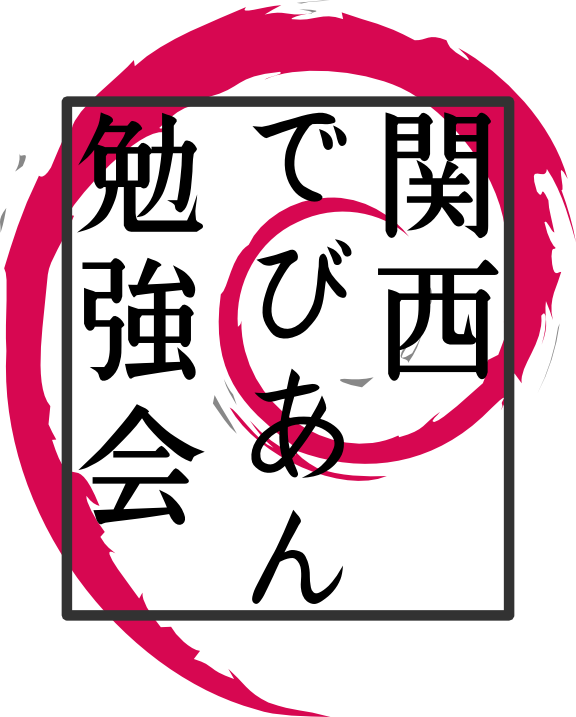
\includegraphics{image200802/kansaidebianlogo.png}
\end{center}

\begin{flushright}
\hfill{}関西 Debian 勉強会担当者 山下 尊也\\
\hfill{}\debmtgyear{}年\debmtgmonth{}月\debmtgdate{}日
\end{flushright}

\thispagestyle{empty}
\end{titlepage}

\dancersection{Introduction}{山下 尊也}
 
 関西 Debian 勉強会はDebian GNU/Linux のさまざ
 まなトピック(新しいパッケージ、Debian 特有の機能の仕組、Debian 界隈で起
 こった出来事、などなど)について話し合う会です。

 目的として次の三つを考えています。
 \begin{itemize}
  \item MLや掲示板ではなく、直接顔を合わせる事での情報交換の促進
  \item 定期的に集まれる場所
  \item 資料の作成
 \end{itemize}

 それでは、楽しい一時をお楽しみ下さい。

\newpage

\begin{minipage}[b]{0.2\hsize}
 {\rotatebox{90}{\fontsize{80}{80}
{\gt 関西デビアン勉強会}}}
\end{minipage}
\begin{minipage}[b]{0.8\hsize}
\hrule
\vspace{2mm}
\hrule
\setcounter{tocdepth}{1}
\tableofcontents
\vspace{2mm}
\hrule
\end{minipage}

%ここから------------------------------------------------------
\dancersection{最近のDebian関係のイベント報告}{山下 尊也}


%ここから------------------------------------------------------
\dancersection{%
Debian を新規に install してから常用環境にするまで \newline
{\normalsize $\sim$ 「chroot から始める sid 」その2 $\sim$}}{佐々木洋平}

\subsection{はじめに}

タイトルのままだと
「アレやソレを install して、 コレを設定して」かと思われるかもしれませんが、
そういう話ではありません%
\footnote{%
それはそれで、別途機会を設けてやりましょうよ。%
{\bf「自分の環境を晒そうよ」}みたいな奴を。}。
ここでは、昨年の関西 Debian 勉強会で尊也さん発表した
「chroot から始める sid」\hcite{山下2008}というネタを膨らませて、
普段は stable を使いながら 
unstable とうまくおつきあいする方法を提案してみます。

「{\bf unstable を常用しないとは。このヘタレめがっ!!}」という声が
どこからともなく聞こえてきそうですが、
いきなり unstable 環境に足を踏み入れるのって結構ドキドキですよね%
\footnote{%
正直な所 unstable を常用するのは佐々木にとってちょっと厳しいです。
だって{\bf 楽しいんだもん}。
やらなきゃイケナイことがあるのに、
美味しそうな餌がそこにある状況はツライです}。

\subsection{chroot ってなんですか?}

簡単に言えば、「コマンドを実行する際に、
実行プロセスおよびその子プロセスのルートディレクトリ({\tt /})を変える」
コマンド(およびそのための関数)です\footnote{%
man (8) chroot, および man (2) chroot 参照。}。
%
ルートディレクトリを別ディレクトリに変更されたプロセスは、
その範囲外のディレクトリにアクセスできなくなります%
\footnote{設定が半端な場合、
やりようによってはアクセスできちゃうみたいですが、%
ここでは触れません。}。
%
chroot を使用する利点は、
カーネル、ハードウェア、ネットワーク、ポート、メモリ空間、プロセス空間等々を
共有したままディレクトリ構造のみを(設定に応じて)切り換えられることです。
VMware や VirutalBox と言った仮想マシン環境の場合には
API やハードウェアのエミュレーションを行ないますが、
これらを行なわない分だけ軽快に動作します。

例えば、
\begin{itemize}
    \item 普段は stable を利用しているけれども、
          特定のプログラムは(最新の) unstable 版を使用したい。
    \item プロプライエタリなソフトウェアが oldstable でしか動かないので、
          そのソフトウェアを oldstable で使用せざるを得ない。
    \item 手元の環境は amd64 なのに、特定のソフトウェアでは i386 のバイナ
          リしか提供されていない。これを使いたい。
    \item パッケージの作成のためのテスト環境に使用する%
          \footnote{{\tt pbuilder} や {\tt piuparts} などに使われています}。
\end{itemize}
といった場合には非常に便利です。

ただし、実際に何らかプログラムを実行する際には、
chroot で変更されたディレクトリ内にライブラリ等が揃っている必要があります。
これを実現するために、
Debian には {\tt cdebootstrap} というパッケージが提供されています。

\subsection{Debian での chroot 環境作成}

では早速{\tt cdebootstrap} を使用して chroot 環境を作成してみましょう。
とりあえず、ここでは
\begin{itemize}
    \item 作業環境(親と呼びます)は stable(=lenny), amd64版
    \item 導入するのは unstable(=sid) amd64版
          \begin{itemize}
              \item chroot の置き場所は {\tt /var/chroot/unstable-amd64}
          \end{itemize}
\end{itemize}
として話を進めます。

先ず cdebootstrap を導入しましょう。
\begin{commandline}
$ sudo aptitude install cdebootstrap
\end{commandline}
次に chroot 環境を作成します。
\begin{commandline}
$ sudo -s
# mkdir -p /var/chroot/unstable-amd64
# cdebootstrap unstable /var/chroot/unstable-amd64 http://ftp.jp.debian.org/debian
...(表示割愛)
\end{commandline}
cdebootstrap によって、
{\tt /var/chroot/unstable-amd64} 以下に unstable の基本システムが展開されます。
実際に chroot で作成した環境に入ってみましょう。
\begin{commandline}
 # chroot /var/chroot/unstable-amd64 
(# chroot /var/chroot/unstable-amd64 /bin/bash   <-- shell が bash 以外の場合には chroot 内で起動する shell を指定する)
\end{commandline}
...無事 chroot されて, unstable 環境に入れたでしょうか?

\subsection{chroot 環境の設定}

この時点では最低限のパッケージしか導入されていないので、
幾つかのパッケージを入れたり抜いたりします。
\begin{commandline}
# vi /etc/apt/sources.list                      <-- contrib, non-free を追記
# aptitude install locales
# dpkg-reconfigure -plow locales
# aptitude update
# aptitude install ~pstandard ~t^japanese$ zsh ... 
...
# aptitude remove nfs-common portmap ....       <-- 不要な物の削除 
\end{commandline}

chroot 環境でパスワードを聞かれそうならば、
/etc/{passwd,shadow} などをコピーしておきます。
\begin{commandline}
$ sudo cp /etc/passwd /var/chroot/unstable-amd64/etc    
sudo sed 's/\([^:]*\):[^:]*:/\1:*:/' /etc/shadow \
  | sudo tee /var/chroot/unstable-amd64/etc/shadow
$ sudo cp /etc/group /var/chroot/unstable-amd64/etc
$ sudo cp /etc/hosts /var/chroot/unstable-amd64/etc
$ sudo cp /etc/sudoers /var/chroot/unstable-amd64/etc
\end{commandline}

また、プロセス空間やデバイスファイルを共有するために
/etc/fstab を修正しておきます。
\begin{commandline}
$ sudo vi /etc/fstab
...(以下を追記)...
/home             /var/chroot/unstable-amd64/home     none    rbind     0   0
/tmp              /var/chroot/unstable-amd64/tmp      none    bind      0   0
proc-sid-amd64    /var/chroot/unstable-amd64/proc     proc    defaults  0   0
devpts-sid-amd64  /var/chroot/unstable-amd64/dev/pts  dev/pts defaults  0   0
\end{commandline}
ここでは chroot の外側で /home 以下に別のファイルシステムをマウントしている場合
でもそれに追従できるようにするために rbind にしています。

fstab に書いた内容を有効にした後に再び chroot 環境下に入ってみましょう。
\begin{commandline}
$ sudo mount -a
$ sudo -s
# chroot /var/chroot/unstable-amd64 
\end{commandline}
/home 以下が chroot 環境下にもマウントされているでしょうか。
ここまでで /var/chroot/unstable-amd64 以下に unstable の環境が整いました。

\subsection{一般ユーザでの chroot 環境の使用}

さて、ここまでは
chroot コマンドを使用して chroot 環境下に入るためには root 権限が必要でした。
一般ユーザの権限でも(設定は必要ですが) chroot を用いて
chroot 環境下のソフトウェアを使用するために、
{\tt schroot }というパッケージが提供されています。

man によれば schroot は
\begin{commandline}
DESCRIPTION

     schroot  allows  the user to run a command or a login shell in a chroot
     environment.  If no command is specified, a login shell will be started
     in the user's current working directory inside the chroot.

     The  command is a program, plus as many optional arguments as required.
     Each argument may be separately quoted.

     The directory the command or login shell is run  in  depends  upon  the
     context.  See --directory option below for a complete description.

     If  the  user is not an allowed user, or a member of the allowed groups
     (or if changing to root, the allowed root users or allowed root groups)
     for  the specified chroot(s), the user will be required to authenticate
     themselves (typically with a password, but this depends  upon  the  PAM
     configuration).  All chroot usage will be logged in the system logs.

     If  no  chroot is specified, the chroot name or alias 'default' will be
     used as a fallback.  This is equivalent to ``--chroot=default''.
\end{commandline}
とあります。

では schroot を導入してみましょう。
\begin{commandline}
$ sudo aptitude install schroot
\end{commandline}
導入したら /etc/schroot/schroot.conf を設定します。
\begin{commandline}
$ sudo vi /etc/schroot/schroot.conf
[unstable-amd64]
description=Debian unstable amd64                 <-- 適当で
location=/var/chroot/unstable-amd64               <-- cdebootstrap で作成した場所を指定
priority=3                                        <-- とりあえず気にならさらず
users=uwabami                                     <-- chroot 環境下に login できるようにする user アカウント
root-users=uwabami                                <-- chroot 環境下に login できるようにする user アカウント
aliases=default,sid                               <-- schroot 実行時の alias
\end{commandline}
description, priority はとりあえず気にしなくても良いです。

以上を設定しておくと、 例えば
\begin{commandline}
$ schroot -c unstable                             <-- chroot 環境へ login
...
$ schroot -c sid                                  <-- aliases で login
...
$ schroot -c unstable -p                          <-- 親の環境変数を引き継いで login
...
$ schroot -c unstable -p xterm                    <-- 直接 chroot 環境下のプログラムを実行]
...
$ schroot -c unstable -p -- xterm -e /bin/sh      <-- option を渡したりできる。
...
$ schroot -c unstable -u root                     <-- root として login
\end{commandline}
なんて事ができるようになります。

\subsection{マウントや/etc/passwod などのコピーを schroot に任せる}

/etc/schroot 以下は次の様になっています。
\begin{commandline}
$ ls -R /etc/schroot
 /etc/schroot:
 chroot.d/  copyfiles-defaults  exec.d/  mount-defaults  schroot.conf  script-defaults  setup.d/
 
 /etc/schroot/chroot.d:
 
 /etc/schroot/exec.d:
 00check*
 
 /etc/schroot/setup.d:
 00check*  05file*  05lvm*  10mount*  15killprocs*  20copyfiles*  50chrootname*
\end{commandline}

/etc/schroot.conf において
\begin{commandline}
type=directory
run-setup-scripts=true
run-exec-scripts=true
\end{commandline}
を追記した後に schroot を実行すると、
proc、dev/pts、/home の bind マウントが自動で行なわれます。
マウント先は {\tt /var/lib/schroot/\$(hash)/} 以下です。
{\tt \$(hash)} は schroot 実行時に自動的に生成されます。
マウントの形式は bind Mount になっています。
また、先程コピーした /etc/\{passwod, shadow\} なども
schroot 実行時に自動的に親環境から copy されます。
copy されるファイルは /etc/schroot/copyfiles-default で設定できます。

run-\{exec,setup\}-scripts=true としておくと
/etc/schroot/\{setup.d, exec.d\} 以下に置いた script を実行してから
chroot 環境下に login することもできます。
なので、ちょっとかわった事をしたい場合にはこのあたりに script を転がしておくと
良いでしょう
(例えば、親環境で mount した光学ドライブを自動で bind マウントする, 等)。

type には {\tt lvm-snapshot} や {\tt block-device} といった設定をすること
もできます。他にも setup.d 以下にファイルを展開するスクリプトを用意しておくと、
chroot 環境を tar.gz で固めて置いておく、なんて事もできます.

\subsection{まとめ}

完全な仮想環境とまではいきませんが、
stable $leftrightallow$
testing $leftrightallow$
unstable (さらに experimental) までをお手軽かつ安全に渡り歩く環境として
chroot と schroot を紹介しました。

schroot は

最近は laptop でも 100 GB 越える HDD が搭載されていたりするので、
試しに unstable/experimental のパッケージを使ってみたい、という場合には
是非試してみて下さい。

最後に、結果として佐々木の /var/chroot 以下はどうなっているかと言うと
\begin{commandline}
$ ls -lh /var/chroot
drwxrwxr-x 2 root root  4.0k 2007-06-26 12:33 etch-amd64/
drwxrwxr-x 2 root root  4.0k 2007-06-26 11:33 etch-i386/
drwxrwxr-x 2 root root  4.0k 2009-04-26 08:32 experimental-amd64/
drwxrwxr-x 2 root root  4.0k 2009-03-01 08:31 lenny-i386/
-rw-rw-r-- 2 root root  9.4G 2005-12-06 11:35 sarge-i386.tar.bz2
drwxrwxr-x 2 root root  4.0k 2009-04-16 12:33 squeeze-amd64/
drwxrwxr-x 2 root root  4.0k 2009-04-18 10:13 squeeze-i386/
drwxrwxr-x 2 root root  4.0k 2009-04-26 08:31 unstable-amd64/
drwxrwxr-x 2 root root  4.0k 2009-04-26 08:31 unstable-i386/
\end{commandline}
なんか自分でも残念な気持になりました。

%------------------------------------------------------
\begin{thebibliography}{99}
    \bibitem[山下, 2008]{山下2008}
                    山下 尊也、2008:
                    chroot からはじめる sid、
                    あんどきゅめんてっど でびあん 2008 夏号、
                    pp. 94 -- 95
    \bibitem[武藤, 2007]{武藤2007}
                    武藤健志、2007:
                    Etch/Sid 上に Sarge 環境を作る方法、
                    {\url http://kmuto.jp/d/index.cgi/debian/debootstrap.htm}
    \bibitem[青木, 2008]{Debianリファレンス}
                    青木 修、角田 慎一(訳)、 
                    Debian リファレンス 8.6.35 chroot、 
                    {\url http://www.debian.org/doc/manuals/reference/index.ja.html}
\end{thebibliography}

%ここから------------------------------------------------------

\dancersection{パッケージの依存性を解く:EDOS から Mancoosi まで}{Ralf Treinen}


注) Ralf Treinen さんの発表用スライドを、簡単かつ適当に抄訳しました。英語が苦手な方は、発表前にざっと読んで内容を把握しておいてください。
訳の間違いなど、苦情は倉敷まで。

\subsection{Mancoosi プロジェクト}

\begin{itemize}
\item ヨーロッパにおける研究プロジェクト
\item 期間:2008/2 → 2011/1
\item EDOS プロジェクト (2004/1 → 2007/6) の後継
\end{itemize}

\subsection{EDOS と Mancoosi の目的}

\begin{itemize}
\item コンピュータサイエンスの研究成果をフリー/オープンソースソフトウェア
      (F/OSS) ディストリビューションに応用:
      \begin{itemize}
          \item 形式手法:論理に基くツールと手法 from Verification
          \item ツール from ソフトウェア工学
      \end{itemize}
    \item F/OSS ディストリビューションと、科学的研究において、
          到達水準を向上させるのが目的
\end{itemize}


\subsection{なぜ科学研究者が F/OSS に興味をもつのか?}

F/OSS インフラストラクチャが特に興味深いのは:
\begin{itemize}
    \item 中心となる設計者がいない
    \item 開発が速く、分散されている
    \item パッケージの相互依存が強い
    \item 巨大なコードベース
    \item 同時に複数の CPU アーキテクチャにパッケージを提供
    \item 複数の OS に対して同時にパッケージを提供
\end{itemize}

\subsection{なぜ F/OSS が科学の研究成果に興味をもつのか?}

F/OSS における品質保証の現状は:
\begin{itemize}
    \item コンパイルとインストールの (時には自動化された) テスト
    \item テストケースの自動生成はなされない
    \item 自動検証ツールは使われていない
    \item 個別のパッケージと、ディストリビューション全体について、
          品質保証のための自動化されたツールが必要に迫られている
\end{itemize}


\subsection{パッケージの依存関係における EDOS workpackage}

焦点:リリース管理者の観点によるディストリビューションの一貫性

質問:規定のリポジトリにあるパッケージしか使えない場合に、ユーザが選択したパッケージはインストール可能だろうか?

リリース管理者や品質保証チームが、問題のある、もしくは無用なパッケージを見つける助けになる質問



\subsection{パッケージのインストーラビリティ as SAT (命題論理の充足可能性判定問題)}

パッケージの関係について、命題論理に基いて数学的なモデルを作ることから始めた。

\begin{itemize}
\item 各パッケージ $p$ (バージョンは $v$) は、ブール変数 $p_v$ 
      ($p_v$ であればパッケージはインストール可能。そうでなければ不可能) 
      として解釈される
    \item 依存関係は、それぞれ連鎖として解釈される。
          例:aterm →
          $\mathrm{libc6}\wedge(\mathrm{libice6}\lor\mathrm{xlibs}) \cdots$
\item パッケージ a と b での衝突は、公式 $!(\mathrm{a}\wedge\mathrm{b})$
      として解釈される
\end{itemize}

定理:

あるパッケージ $p$ のバージョン $v$ は、$p_v$ を真とする真偽値が存在し、
リポジトリの記号化を満足すれば、「インストール可能」である


\subsection{パッケージインストールの容易さ as SAT − 例}


平均的な式は 400 の定数を持つ。KDE のインストールでは 32000


\subsection{EDOS ツールチェイン}

EDOS を通じていくつかのツールが開発された (OCaml で 110000 行のコード)

\begin{description}
\item[edos-debcheck] \mbox{}

パッケージのインストーラビリティをチェックするコマンドラインツール
\item[pkglab] \mbox{}

インタラクティブなコンソール環境で、リポジトリの検査用
\item[ceve] \mbox{}

パッケージリストの複数フォーマットをパース/変換する
\item[tart] \mbox{}

リポジトリを分割 (メディアなど) する。この時、i 番目のメディアに含まれているパッケージは、i 番目までのメディアを使えばインストール可能となる
\end{description}

いくつかを詳細に見てみよう……


\subsection{edos-debcheck}

\begin{itemize}
\item edos-debcheck は APT パッケージリスト (/var/lib/apt/lists/* など) をもとに、ある/いくつかの/全てのパッケージがインストール可能かどうかをチェックする
\end{itemize}

カスタマイズされた SAT 解決器がベースになっていて、とても高速:testing/amd64 の main にある全パッケージのインストーラビリティのチェックにかかる時間は、エントリーレベルのマシン上で 5 秒。

\begin{description}
\item[大きな成功例] \mbox{}

emdebian ではパッケージのアップロード前に edos-debcheck を使って、壊れたパッケージをアーカイブにアップロードしないようにしている
\end{description}

Debian のパッケージ名:edos-debcheck, edos-rpmcheck


\subsection{pkglab}

pkglab はインタラクティブな、コンソールベースの環境で、パッケージベースのソフトウェアディストリビューションのリポジトリを調査するもの

機能:

\begin{itemize}
\item 現在と過去のパッケージリストを読み込む
\item パッケージのインストーラビリティをチェック (edos-debcheck で)
\item 関数型のクエリ言語 (map, filter, fold, \dots{})
\item リポジトリがどのような変遷を経て発展してきているかを調べる (edos-debcheck 単体では不可能)
\end{itemize}

Debian のパッケージ名:dose2 (基本のライブラリ), ceve (パッケージリストのパーサ/コンバータ), pkglab (インタラクティブ環境), edos-debcheck (debian 向けのインストーラビリティチェッカ), edos-rpmcheck (RPM 向けのインストーラビリティチェッカ)


\subsection{Debian で、インストールできないパッケージを見つける}

Debian, Skilelinux, Debian GNU/kFreeBSD において、毎日 edos-debcheck を使ってインストール不可能なパッケージをモニターしている:

\url{http://edos.debian.net/edos-debcheck}

インストールできないパッケージの頻出ケース:

\begin{enumerate}
\item autobuilder の追随 (例えば、arch:all のパッケージが arch:any のパッケージと同時にアップロードされ、autobuilder が遅延している):通常の一過性のインストール不可状態
\item a が b に依存しており、全アーキテクチャに b がない:b のビルドに問題があったり、a において、とってもおおらかなアーキテクチャ指定がなされている (厳密にすべき)

\begin{itemize}
\item 上記の特殊な例:a は arch:all。最近のInstall-To フィールドを追加する提案はこれに対処するもの (\#436733)
\end{itemize}
\item 深刻なパッケージのバグで、実際に修正する必要がある :-)
\end{enumerate}


\subsection{Debian で、宣言されていない衝突を見つける}

ユーザにこういったエラーを見せる前に取り除く。

\begin{enumerate}
\item 愚直に:パッケージ全部 (200,000,000) を同時にインストールしてみる……そんなバカな!
\item 少なくとも 1 ファイルを共有しているペアのみ考慮 (Contents を使えば簡単):867 ペア (2008/4/16 の amd64/sid)
\item 依存性のうえで同時インストール可能なペアに絞る (pkglab を使えば簡単):102 ペア
\item diversion によって誤検知されているかも:ペアでのインストールを chroot 環境でテスト:27 のバグもちパッケージペアが検出された
\end{enumerate}

レポート:\url{http://edos.debian.net/missing-conflicts/}

BTS:ユーザ \verb|treinen@debian.org|、タグ edos-file-overwrite


\subsection{Mancoosi プロジェクト}

アップグレード問題 = インストールされたパッケージのローカルなステータスを変更するようメタインストーラが要求することで発生する問題。

アップグレード問題の解決は、いくつかの理由で失敗し得る:

\begin{itemize}
\item 呼び出しエラー、依存性解決、パッケージ受信、パッケージ展開、メンテナスクリプトの実行、……
\end{itemize}

Mancoosi は 2 つの側面からアップグレード問題に取り組もうとしている:

\begin{description}
\item[ロールバックのサポート] \mbox{}

想定外のエラー (メンテナスクリプトなど) があった場合、事後のリカバリが唯一の解決策
\item[依存性解決] \mbox{}

メタインストーラが最新の水準を満たしていない (例えば、不完全性:when there is one、解決法を見つけることができない):我々がうまくやらねば!
\end{description}


\subsection{依存性の解決に必要なもの}

\begin{description}
\item[完全性] \mbox{}

アップグレード問題への解決法が存在するなら、メタインストーラはそれを発見できなくてはならない
\item[最適性] \mbox{}

同等の異なる複数の解決法を区別するため、最適化の基準を指定できる必要がある。例えば:
\end{description}

\begin{itemize}
\item ダウンロードサイズを最小化
\item 使用するディスクスペースを最小化
\item J. Random DD (DD の誰か) がメンテしているパッケージのブラックリスト
\item などなど
\end{itemize}

\begin{description}
\item[効率] \mbox{}

依存性の解決は、可能な限り高速でなくてはならない
\end{description}


\subsection{依存性解決法の competition}

我々は、依存性解決における魔法の銀の弾丸となるアルゴリズムを探そうとしているわけではもちろんないが、依存性解決の competition 運営につながる助けとなることができる

\begin{itemize}
\item popcon のように収集した現実におけるアップグレード問題 (メタインストーラが持つオプトインのデータ収集プラグイン)
\item 様々な証跡:平易な分析 (スピード)、最適化した分析 (よりよい解法)、……
\item 開発者と研究者が、独自アルゴリズムの独自実装を提示することができる
\item 勝者は幸運と栄光をゲット
\end{itemize}

SAT 解決自体のような関連分野において、同様の competition が技術水準を最新に押しあげるのに大いに寄与しています。なぜこの分野でやらないのでしょう?



%ここから------------------------------------------------------

\dancersection{今後の予定}{山下 尊也}

\subsection{次回}
次回は、2009年 5 月 31 日に福島区民センターで行います。

% 冊子にするために、4の倍数にする必要がある。
% そのための調整
% \dancersection{メモ}{}
% \mbox{}\newpage
% \mbox{}\newpage

\printindex
 \cleartooddpage

 \begin{minipage}[b]{0.2\hsize}
  \rotatebox{90}{\fontsize{80}{80} {\gt 関西デビアン勉強会} }
 \end{minipage}
 \begin{minipage}[b]{0.8\hsize}

 \vspace*{15cm}
 \rule{\hsize}{1mm}
 \vspace{2mm}
 
\includegraphics[width=2cm]{image200502/openlogo-nd.eps}
 \noindent \Large \bf Debian 勉強会資料\\ \\
 \noindent \normalfont \debmtgyear{}年\debmtgmonth{}月\debmtgdate{}日 \hspace{5mm}  初版第1刷発行\\
 \noindent \normalfont 関西 Debian 勉強会 (編集・印刷・発行)\\
 \rule{\hsize}{1mm}
 \end{minipage}

\end{document}
